%http://distro.ibiblio.org/smeserver/contribs/gordonr/devguide/html/c1115.htm
%http://www.sme-server.de/download/Howtos/Customizing_SME.html
%https://wiki.contribs.org/SME_Server:Documentation:Developers_Manual

La arquitectura interna del SME Server se basa en cuatro componentes:

\begin{itemize}
\item Interfaces de administración, tanto por consola como web.
\item Bases de datos de configuración.
\item El sistema de templates, que es usado para generar archivos de configuración.
\item Eventos y acciones.
\end{itemize}

Cuando un usuario configura alguno de los aspectos del servidor, la máquina configura automáticamente las aplicaciones que son relevantes a ese cambio. Esto se realiza en varios pasos:
\begin{itemize}
\item La interfaz de usuario cambia valores en las bases de datos de configuración. En estas bases de datos se almacena información que describe el estado del sistema, como las asignaciones de direcciones IP, los nombres de dominio, las cuentas de usuario...
\item Después de haber cambiado estos valores, la interfaz de usuario envía una señal de evento para realizar los cambios en las aplicaciones. Por ejemplo, si hacemos cambios en la configuración del email, el evento que se señala es el 'email-update'. Estos eventos son colecciones de scripts, que se ejecutan en un orden determinado para producir las modificaciones deseadas.
\item Estos scripts actualizan los ficheros de configuración de las aplicaciones. Los generan usando las templates, que no son más que plantillas usadas para este propósito. Los scripts de actualización leen las bases de datos de configuración, de manera que los nuevos archivos generados contienen nuestras últimas modificaciones.
\item Por último las aplicaciones son avisadas de que su configuración ha sido cambiada, por lo que releen los archivos o se reinician, según convenga.
\end{itemize}

Aquí tenemos una imagen que describe este proceso:

\begin{figure}[H]
    \centering
    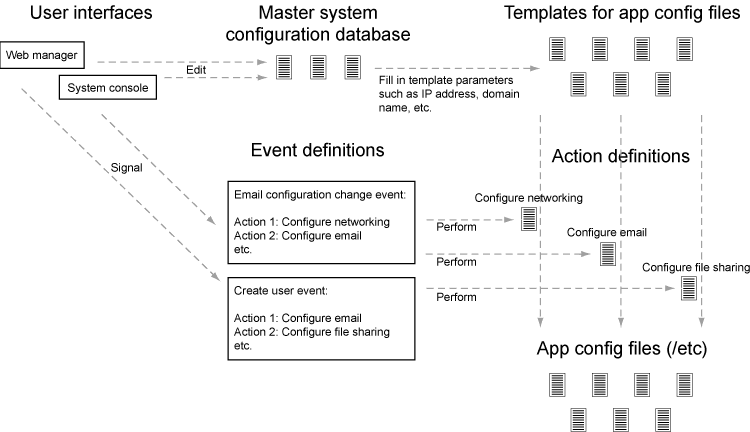
\includegraphics[width=\textwidth]{arquitectura/Sme-server-architecture.png}
%    \caption{Arquitectura interna del SME server}
\end{figure}

\section{Bases de datos de configuración}
Todos los parámetros de configuración que son modificables por el usuario son almacenados aquí. Las entradas pueden ser de dos tipos:
\begin{itemize}
\item Simples: constan de un par clave/valor.
\begin{figure}[H]
    \centering
    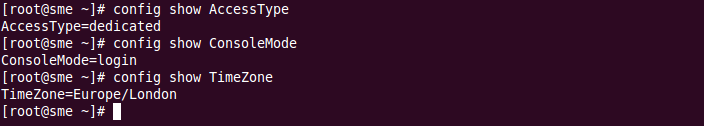
\includegraphics[width=\textwidth]{arquitectura/01.png}
%    \caption{Entradas simples}
\end{figure}
\item Complejas: constan de una clave, un tipo y una colección de pares propiedad/valor.
\begin{figure}[H]
    \centering
    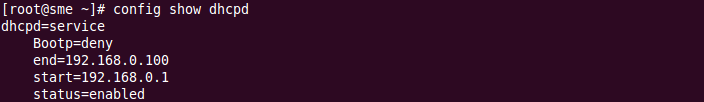
\includegraphics[width=\textwidth]{arquitectura/02.png}
%    \caption{Entradas complejas}
\end{figure}
\end{itemize}

\subsection{Acceso a las bases de datos}

\begin{itemize}
\item \textbf{Acceso mediante la línea de comandos}
\end{itemize}
El comando para acceder a los datos de las bases de datos de configuración es \lstinline!db!. Podemos ver una pequeña ayuda tecleando \lstinline!db! sin más:
\begin{figure}[H]
    \centering
    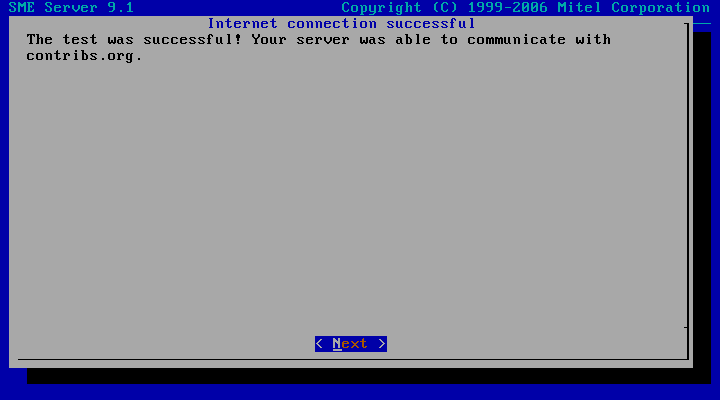
\includegraphics[width=\textwidth]{arquitectura/03.png}
\end{figure}

Las bases de datos existentes son \lstinline!accounts!, \lstinline!networks!, \lstinline!configuration!, \lstinline!domains! y \lstinline!hosts!. Además, tenemos el comando \lstinline!config show!, que es un alias para \lstinline!db configuration show!.

\begin{figure}[H]
    \centering
    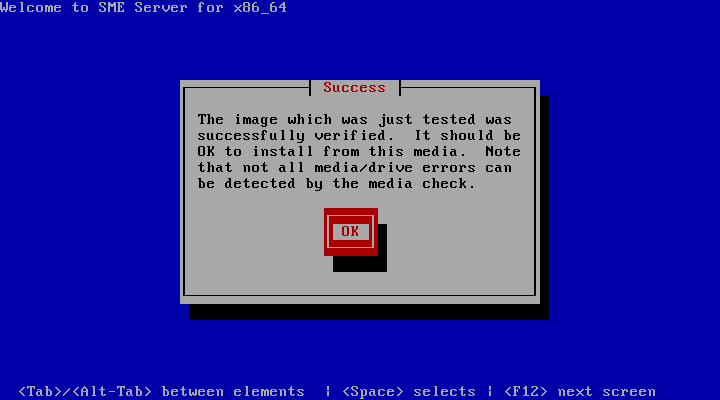
\includegraphics[width=\textwidth]{arquitectura/04.png}
\end{figure}

\begin{itemize}
\item \textbf{Acceso desde un script de Perl}
\end{itemize}

SME Server incorpora una API para Perl para acceder a las bases de datos de configuración. Para ver ayuda y ejemplos, podemos acceder a la documentación usando el comando \lstinline!perldoc!:

\begin{lstlisting}
  perldoc esmith::ConfigDB
  perldoc esmith::AccountsDB
  perldoc esmith::HostsDB
  perldoc esmith::NetworksDB

  perldoc esmith::DB
\end{lstlisting}

%Esto está comentado
\begin{comment}
Script para consultar el usuario admin:

\begin{lstlisting}[language=Perl,style=perlo]
#!/usr/bin/perl -w
  
use esmith::AccountsDB;

my $db = esmith::AccountsDB->open or die "No se puede abrir la BD Accounts\n";

my $admin = $db->get("admin") or die "No existe la cuenta admin en la BD ACcounts\n";

print $admin->show();
\end{lstlisting}
\end{comment}
%%%%%%%%%%%%%%%%%%%

%----------------------------------------------------------
%
%         ACCIONES Y EVENTOS
%
%----------------------------------------------------------
\section{Acciones y eventos}

\subsection{Acciones}

Una acción es un programa que ejecuta una única tarea, como editar un archivo de configuración o reconfigurar un servicio. Las acciones son llamadas marcando un evento, nunca directamente. Están en el directorio \lstinline!/etc/e-smith/events/actions!.

\begin{figure}[H]
    \centering
    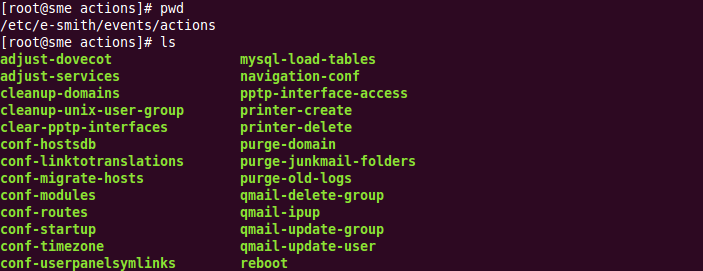
\includegraphics[width=\textwidth]{arquitectura/05listaActions.png}
\end{figure}

\subsection{Eventos}

Los eventos son un mecanismo que permite al sistema ejecutar una serie de acciones en respuesta a un cambio. Están asociados a una lista de acciones que se ejecutan en un orden determinado. Se encuentran en la carpeta \lstinline!/etc/e-smith/events!\\

Por ejemplo, en el caso de un cambio de la dirección IP externa, se llamaría al evento \lstinline!ip-change!. Este evento se compone de lo siguiente:

\begin{figure}[H]
    \centering
    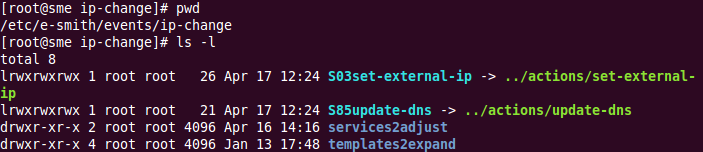
\includegraphics[width=\textwidth]{arquitectura/06eventoIp.png}
\end{figure}

\begin{itemize}
\item Enlaces simbólicos a dos acciones, una que escribe la nueva IP externa en la base de datos \lstinline!configuration! y otra que actualiza el servicio de DNS dinámico que tuviéramos configurado con la nueva IP de nuestra máquina. El prefijo que llevan los links sirve para establecer en qué orden se ejecutarán. Este es el cuerpo del script que cambia la IP externa:
\end{itemize}

\begin{figure}[H]
    \centering
    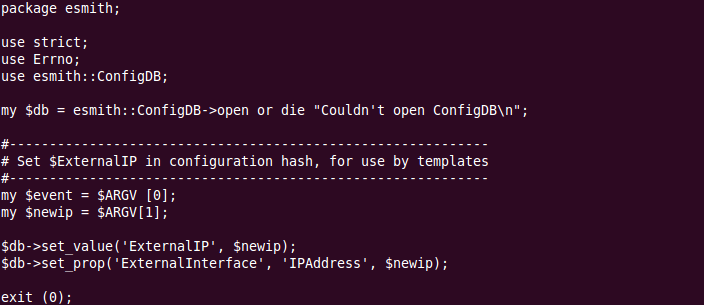
\includegraphics[width=\textwidth]{arquitectura/07set-external-ip.png}
\end{figure}

Aquí podemos ver cómo se usa el API de Perl para acceder a la base de datos \lstinline!configuration! y cambiar valores. Casi todas las acciones son llamadas siempre con 2 argumentos: el nombre del evento que las ha llamado y el nuevo valor que se va a asignar. La IP externa del equipo es guardada en 2 registros diferentes de esta base de datos, por razones de compatibilidad con versiones anteriores de SME server:

\begin{figure}[H]
    \centering
    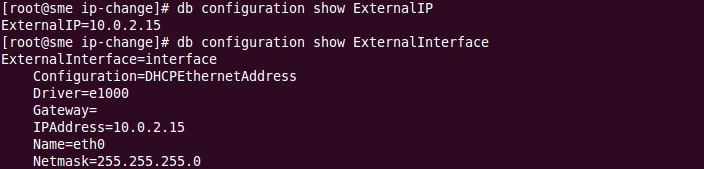
\includegraphics[width=\textwidth]{arquitectura/08extInterfaceEnBD.png}
\end{figure}

\begin{itemize}

\item Acciones implícitas. La mayoría de eventos contienen dos tareas comunes: expandir los templates necesarios y reajustar los servicios implicados. Para ello se ejecutan las acciones \lstinline!generic_template_expand! y \lstinline!adjust-services!, cuyo código se encuentra en \lstinline!/etc/e-smith/events/actions!. Los subdirectorios que encontramos en la carpeta de nuestro evento son usados por estas dos acciones:

\begin{itemize}

\item[-] Directorio \lstinline!services2adjust!, para la acción \lstinline!adjust-services!. Contiene links de los servicios que se tienen que reajustar y la acción que se debe efectuar sobre ellos.

\begin{figure}[H]
    \centering
    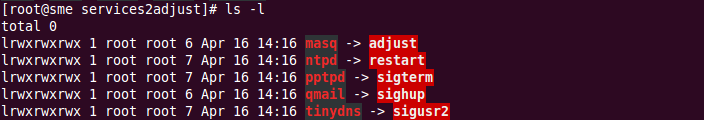
\includegraphics[width=\textwidth]{arquitectura/09services2adjust.png}
\end{figure}

\item[-] Directorio \lstinline!templates2expand!. Lista de los archivos de configuración que tienen que volver a ser regenerados desde las plantillas.

\begin{figure}[H]
    \centering
    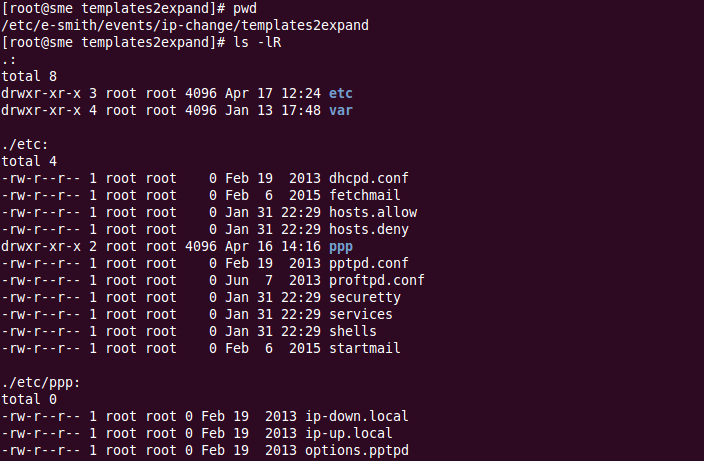
\includegraphics[width=\textwidth]{arquitectura/10templates2expand.png}
\end{figure}
\end{itemize}
\end{itemize}

Por defecto, la acción \lstinline!generic_template_expand! se ejecua con prioridad S05, y la acción \lstinline!adjust-services! con S90. Por ello se recomienda que las acciones propias que queramos incluir estén entre S10 y S80. Sabiendo esto podemos comprender el orden en el que se ejecutan las acciones en nuestro ejemplo, el evento de cambio de IP externa:
\begin{enumerate}
\item Se cambia el valor de IP externa en la base de datos de configuración.
\item Se actualizan los archivos de configuración de los servicios y programas implicados.
\item Si tenemos configurado servicio de DNS dinámico, se actualiza (se advierte al servidor de nuestro cambio de IP).
\item Se reconfiguran todos los servicios con la nueva IP.
\end{enumerate}

\subsection{Señalar un evento}
Para ejecutar todas las acciones de un evento usamos el comando \lstinline!signal-event!, seguido del nombre del evento. Este comando además escribe todo el output en el log del sistema \lstinline!messages!.

\begin{lstlisting}
  signal-event ip-change 216.58.210.35
\end{lstlisting}

El comando \lstinline!signal-event! no suele tener más argumentos que el nombre del evento, ya que en general se prefiere hacer los cambios en los archivos de configuración antes de llamar al evento.

%%%%%
\begin{comment}
\subsection{Eventos importantes}

\begin{longtable}{p{0.15\textwidth} |p{0.15\textwidth} | p{0.61\textwidth} }
  \textbf{Evento} & \textbf{Argumento} & \textbf{Descripción}\\\hline
  \lstinline!aaa! & - & bbb\\
\end{longtable}
\end{comment}
%%%%%

%----------------------------------------------------------
%
%         TEMPLATES
%
%----------------------------------------------------------

\section{Templates}

El sistema de templates (plantillas) presente en SME server sirve para generar los archivos de configuración de las aplicaciones. Proporciona un método uniforme para cambiar estos archivos, sin tener que preocuparnos de la sintaxis particular que usa cada uno. De hecho, en SME server no debemos editar nunca los archivos de configuración a mano, ya que se sobreescribirán con los generados por las plantillas en algunas situaciones, por ejemplo si activamos algún evento que requiera el ajuste de esas aplicaciones, o si reiniciamos del sistema.\\

Las templates se encuentran en el directorio \lstinline!/etc/e-smith/templates!.

\begin{figure}[H]
    \centering
    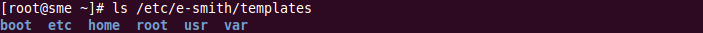
\includegraphics[width=\textwidth]{arquitectura/11templates.png}
\end{figure}

Aquí nos econtramos una estructura de directorios que se corresponde con la del sistema. Por ejemplo, la template para \lstinline!/etc/hosts! estará en \lstinline!/etc/e-smith/templates/etc/hosts!.\\

Las plantillas están almacenadas en \textbf{fragmentos}. Es decir, en nuestro ejemplo, \lstinline!/etc/e-smith/templates/etc/hosts! no es un archivo sino un directorio con diferentes archivos. Estos fragmentos se concatenan según el orden ASCII de sus nombres, y el archivo resultante es el que se encarga de generar el archivo de configuración de la aplicación.

\begin{figure}[H]
    \centering
    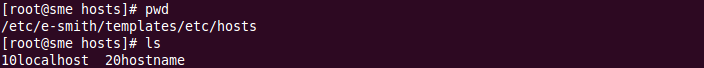
\includegraphics[width=\textwidth]{arquitectura/13hosts.png}
\end{figure}

La plantilla para \lstinline!/etc/hosts! es fácil de entender.

\begin{figure}[H]
    \centering
    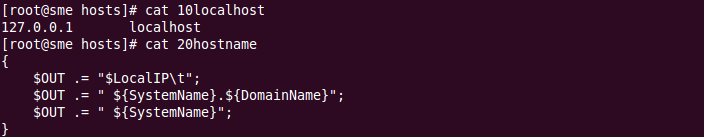
\includegraphics[width=\textwidth]{arquitectura/14hosts.png}
\end{figure}

El primer archivo contiene texto, que se añade sin más al archivo de configuración. El segundo archivo contiene un pequeño script de Perl (todo lo que va entre llaves se ejecuta), que usa valores de la base de datos de configuración.\\

\subsection{Expansión de templates}

Para regenerar los archivos de configuración cuya plantilla hemos modificado, debemos expandir esa plantilla:

\begin{lstlisting}
  expand-template /etc/archivo.conf
\end{lstlisting}

También debemos reiniciar el servicio en cuestión. Se puede hacer con el siguiente comando:

\begin{lstlisting}
  sv t /ruta/del/servicio
\end{lstlisting}

Algunos eventos combinan la expansión de ciertas plantillas y el reinicio de todos los servicios afectados. Por ejemplo, si modificamos algo en la configuración del email, llamaremos al siguiente evento:

\begin{lstlisting}
  signal-event email update
\end{lstlisting}

Si dudamos qué templates debemos expandir o qué servicios debemos reiniciar, podemos marcar los siguientes eventos, que expandirán todas las plantillas y reiniciarán el sistema:

\begin{lstlisting}
  signal-event post-upgrade
  signal-event reboot
\end{lstlisting}

\section{Ejemplo práctico: php.ini}

Si queremos modificar una de las templates o fragmentos que vienen presentes en la distribución, deberemos copiarla, junto con la estructura de directorios adecuada, desde \lstinline!/etc/e-smith/templates! a \lstinline!/etc/e-smith/templates-custom!, y editarla aquí. En caso de que exista una template en cada uno de estos dos directorios con el mismo nombre, solo se usará la de \lstinline!templates-custom!. Esto es así para que en el caso de que cometamos algún fallo podamos revertir el cambio fácilmente, sin más que borrar la plantilla en \lstinline!templates-custom!. Si queremos introducir una template nueva, la crearemos en \lstinline!templates-custom!, con el nombre adecuado, teniendo en cuenta que luego se concatenará con las demás (también las de \lstinline!/etc/e-smith/templates!) según el orden ASCII de sus nombres.\\

Veamos el aspecto que tiene el archivo \lstinline!/etc/php.ini! en el sistema:

\begin{figure}[H]
    \centering
    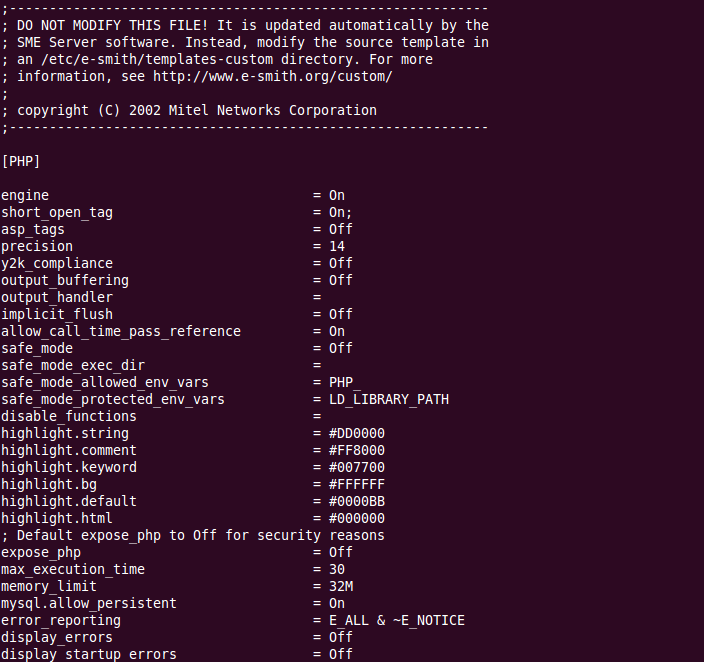
\includegraphics[width=\textwidth]{arquitectura/15phpIni.png}
\end{figure}

Supongamos que queremos cambiar el valor de la directiva \lstinline!display_errors! a \lstinline!On!. Debemos buscar la plantilla, dentro de \lstinline!/etc/e-smith/templates!, en la que se encuentra esta directiva.

\begin{figure}[H]
    \centering
    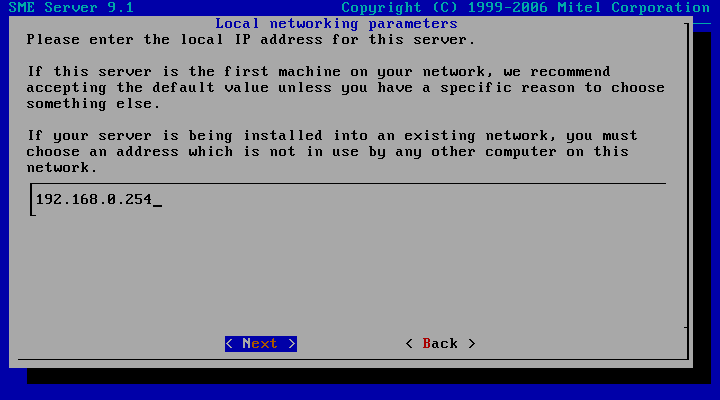
\includegraphics[width=\textwidth]{arquitectura/16.png}
\end{figure}

Copiamos este fragmento de plantilla en el directorio \lstinline!/etc/e-smith/templates-custom/etc/php.ini! (lo creamos si no existía) y lo modificamos allí, cambiando la directiva a \lstinline!On!. Así es como queda:

\begin{figure}[H]
    \centering
    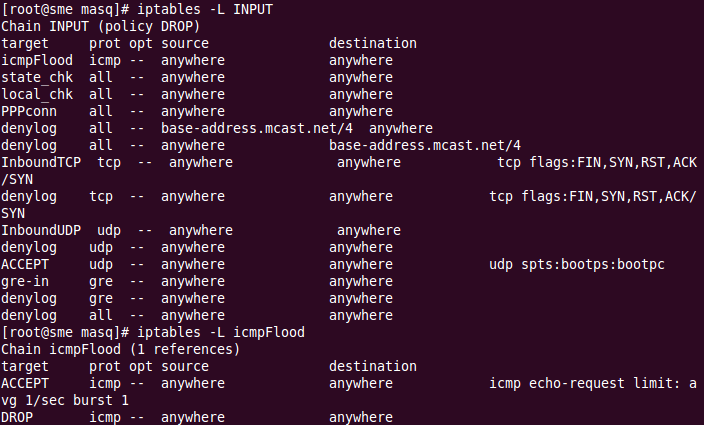
\includegraphics[width=\textwidth]{arquitectura/17.png}
\end{figure}

Para que se modifique el \lstinline!php.ini! real, tenemos que expandir la plantilla y reiniciar el servicio \lstinline!httpd-e-smith!, que es el servidor web.

\begin{lstlisting}
  expand-template /etc/php.ini
  sv t /service/httpd-e-smith
\end{lstlisting}

Podemos ver que el cambio se ha realizado correctamente:

\begin{figure}[H]
    \centering
    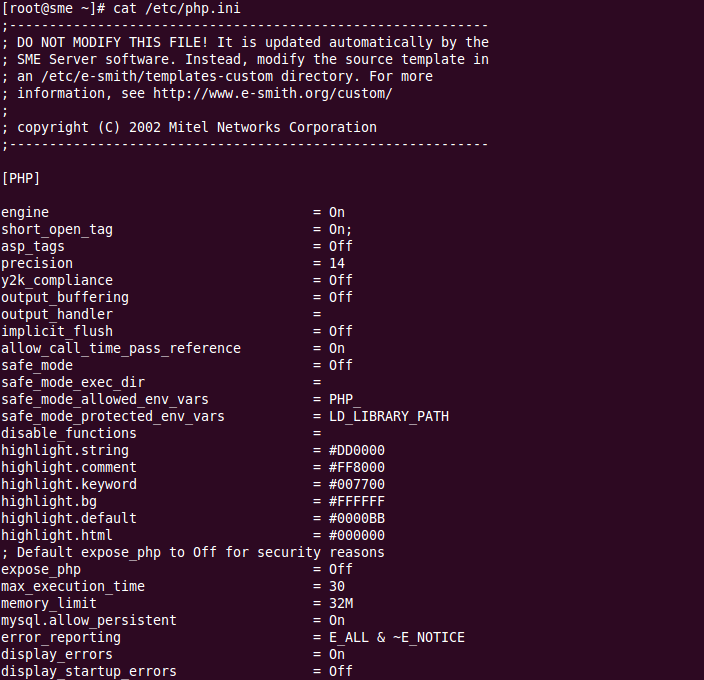
\includegraphics[width=\textwidth]{arquitectura/18.png}
\end{figure}
